\exercises

\exercise 用芝诺时计算阿基里斯的速度$v_1'$和加速度$a_1'$,并给出$x-t'$图。

\exercise 甲乙两列火车在同一水平直路上以相等的速率(30公里/时)
相向而行。当它们相隔60公里的时候,一只鸟以60公里/时的
恒定速率离开甲车头向乙车头飞去,一当到达立即返回,如此来
回往返不止。试求:

(1)当两车头相遇时,鸟往返了多少次?

(2)鸟共飞行了多少时间及距离?

(3)我们定义一种特殊的“小鸟钟”:小鸟从一车头到另一车
头为小鸟钟的时间测量单位(即小鸟钟的一个“滴答”)。用小鸟
钟记时的数值为$t''$求$t''$与一般时钟记时$t$之间的变换。

\exercise 一人从$O$点出发,向正东走3.0米,又向正北走1.0米,
\begin{wrapfigure}[8]{r}{8.5em}
    \begin{center}
        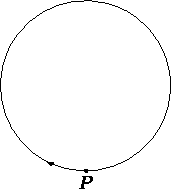
\includegraphics{figure/fig01.28}
        \caption{}
        \label{fig:01.28}
    \end{center}
\end{wrapfigure}
然后向东北走2.0米,试求合位移的大小及方向。

\exercise 一质点从P出发,向左以匀速率1.0厘米/秒沿半径为$R=1.0$米的圆周运动(图\ref{fig:01.28})。问:

(1)当它走过2/3圆周时,位移是多少?走过的路程是多少?在这段时间内的
平均速度是多少?该点的瞬时速度是多少?

~\vspace{-3em}

(2)当它走过1/2圆周时,以上各值又如何?

\exercise 一物体作直线运动,它的位置由方程$x=10t^2+6$决定,其
中$x$的单位为厘米,$t$的单位为秒,试计算:

(1)在3.00~3.10秒、3.000~3.01秒及3.000~3.001秒间
隔内的平均速度,

(2)在$t=3.00$秒时的瞬时速度;

(3)用微分方法求它的速度及加速度公式。

\exercise 有一质点沿x方向作直线运动,t时刻的坐标为:\\
\null\qquad\qquad \qquad $x=4.5t^2-2t^3$\\
式中$x$的单位为米。$t$的单位为秒。试求:

(1)第2秒内的位移和平均速度;

(2)第1秒末和第2秒末的瞬时速度;

(3)第2秒内质点所走过路径的长度;

(4)第2秒内的平均加速度以及第0.5秒末和第1秒末的瞬时
加速度。

\exercise 一质点以恒定的径向速度$r=4$米/秒在一平面中运动。它
的角速度为常量,其大小为$\omega=\dot\theta=2$弧度/秒。当质点距原点为3
米时,它的速度的大小及加速度大小是多少?

{
\exercise 如图\ref{fig:01.29}~所示,向上抛一物体,测量物体上抛及下落经
\begin{wrapfigure}[8]{r}{12.5em}
    \vspace{1em}
    \begin{center}
        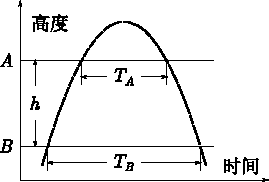
\includegraphics{figure/fig01.29}
        \caption{}
        \label{fig:01.29}
    \end{center}
\end{wrapfigure}
过水平线$A$的时差$T_A$,以及上抛
及下落经过水平线$B$的时差$T_B$。
试证明,若忽略空气阻力,重力
加速度的大小可以表示为:\\
\null\qquad \qquad$g=\dfrac{8h}{T_A^2 - T_B^2}$ \\
式中$h$是$B$线与$A$线的高度差。}

\exercise 天体物理常涉及大尺度的\\
问题,为了方便起见,引进一些
\clearpage
\noindent 实用的大的长度单位。一个天文单位(AU)等于从地球到太阳的
平均距离;一个秒差距是一个天文单位所张之角为1秒的距离,即
观测者从某一恒星看地球公转轨道半径所张的角度为1秒时,该恒
星与太阳之间的距离。试求。

(1)1秒差距相当于多少米?多少天文单位?及多少光年?

(2)以秒差距为单位,表示地球到太阳的距离。

\exercise 一物体从离地面的高度为h的地方,由静止开始自由下
落,经过最后196米所用的时间是4.0秒钟。求物体下落过程所用
的总时间及其高度。

\exercise 一枚从地面发射的火箭以20米/$\text{秒}^2$的匀加速度竖直上升
半分钟后,燃料用完,于是象一个自由质点一样运动。略去空气
阻力,试求。

(1)火箭达到的最大高度;

(2)它从离开地面到再回地面所经过的总时间。

\exercise 把两个小物体从同一地点以同样初速率$v_0=24.5$米/秒
先后竖直上抛,设抛出两物体的时差为$\Delta t=0.500$秒,试问:

\renewcommand{\hsp}{\hspace{0.2em}}
{(1)\ziju{-0.015}第二个物体抛出后,经过多少时间\hsp $t$\hsp 才与第一个物体相遇?}

\vspace{-0.15em}(2)如果$\Delta t\geqslant\dfrac{2v_0}{g}$,讨论结果的物理意义。\vspace{-0.15em}

\exercise 物体以初速$v_0=20$米/秒被抛出,抛射仰角是\ang{60;;},略去
空气阻力,试问:

(1)物体开始运动后的1.5秒束,运动方向与水平方向的夹角
$\alpha$是多少?2.5秒末夹角$\alpha$又为多少?

(2)物体抛出后经过多少时间,运动方向才与水平成\ang{45;;}角?
这时物体的高度是多少?

(3)在物体轨迹最高点处的曲率半径$R_1$有多大?

(4)在物体落地点处,轨迹的曲率半径$R_2$有多大?

\exercise 高台下降滑雪在一平滑的山坡上进行。山坡与水平线成
恒定角度$\alpha$,滑雪运动员初速率为$v_0$,并以与水平线成$\theta$的仰角跳
出(\ref{fig:01.30})。若不考虑空气阻力,试证明:
\begin{figurex}
    \centering
    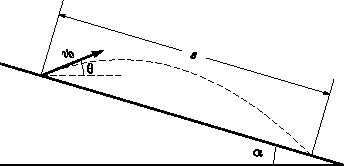
\includegraphics{figure/fig01.30}
    \caption{}
    \label{fig:01.30}
\end{figurex}

(1)运动员落在斜坡上的距离为:
\begin{equation*}
    s=\frac{2 v_{0}^{2} \sin (\theta+a) \cos \theta}{g \cos ^{2} \alpha}
\end{equation*}

(2)对于一定的$v_0$和$\alpha$来说,$s$在$\theta=\ang{45;;}-\dfrac{\alpha}{2}$时有最大值。其
值为:
\begin{equation*}
    s_{\max }=\frac{v_{0}^{2}(1+\sin \alpha)}{g \cos ^{2} \alpha}
\end{equation*}

\exercise 1977年中国男子铁饼的最好记录是54.28米,1983年提高
到60米。这些记录都是在北京创造的,北京的重力加速度$g$为
980.12厘米/$\text{秒}^2$。设投掷点比落地点高1.5米,略去空气阻力,
问投掷时至少要用多大的初速度,才可达到上述距离?

\exercise 设若干个光滑斜面($a_1$,$a_2$,$a_3$,…)有共同的底边$b$为30
厘米。试问:

(1)斜面与水平夹角$\alpha$为多大时,才能使物体在该斜面上从顶
端自由滑至底上正好需时为$t=0.4$秒?

(2)多大的夹角$\alpha$,使下滑的时间最短?

\exercise 在空间某一点$O$以相同的速率向各方向同时把若干小
球搬出去。试证明在略去空气阻力的情况下,任一时刻$t$,所有小
球都位于一个球面上,并求:

(1)此球心的运动方程式;

(2)球面距球心的距离。

\exercise 若抛射体的初速率为$v_0$,抛射角为$\theta$,略去空气阻力。伽
利略说:“抛射角为$\ang{45;;}+\delta$和$\ang{45;;}-\delta(\delta<\ang{45;;})$的两个抛射体初速
率相同时,射程是相等的。”试证明他的话,并证明$\theta=\ang{45;;}$时水
平射程最大。

\begin{wrapfigure}[8]{r}{12.5em}
    \vspace{-2.5em}
    \begin{center}
        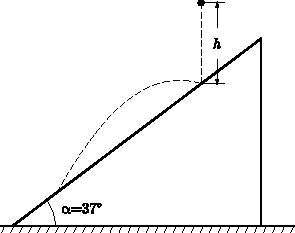
\includegraphics{figure/fig01.31}
        \caption{}
        \label{fig:01.31}
    \end{center}
\end{wrapfigure}
\exercise 一弹性球自由下落在一斜面上,与斜面发生完全弹性碰
撞,下落高度$h=20$厘米,斜面对水平的倾角$\alpha=\ang{37;;}$(图\ref{fig:01.31})。若
不计空气阻力,它第二次碰到斜面的位置距原来的下落点多远?

\exercise 用枪瞄准空中的靶,当子弹射出枪口时,靶同时自由下
落。如果略去空气阻力。不论子弹速率多大,总会击中下落的靶,
这个现象叫做百发百中,说明其中理由。

\exercise 一轰炸机高海面10公里,以240公里/小时的水平速度追
击正前方一鱼雷艇,鱼雷艇的速度是95公里/小时,不计空气阻
力,问飞机应在艇后多少距离投弹才能正好击中目标?

\exercise 一俯冲轰炸机沿与铅垂线成$\ang{37;;}$方向俯冲,在800米高度
投弹,炸弹离开飞机5.0秒钟时着地。不计空气阻力,试问:

(1)飞机的飞行速度是多少?

(2)炸弹离开飞机后在水平方向前进多远?

(3)炸弹着地时,速度的大小和方向?

\exercise 应以多大的水平速度$v$把一物体从高$h$处抛出,才能使
它在水平方向的射程为$h$的$n$倍?

\exercise 飞机以360公里/小时的速度由东向西飞行。试回答:

(1)在什么地理纬度上,飞机上的人可以看见太阳不动地停
在空中?

(2)若在极地附近沿纬线以圆轨道由东向西飞行,可以看见
什么现象?

\exercise 一俯冲轰炸机以不变的速率450公里/小时俯冲后。急离
俯冲线改为沿一铅垂平面内的圆形路线飞行。试问:要使飞机在
圆的最低点的加速度不超过$7g$,圆形路线的最小半径应是多少?

\exercise 车轮在地平面上作匀角速的纯滚动,轮行的速度为$v_0=
10$米/秒,轮的半径为$r=0.50$米,试求;

(1)车轮边缘上一点$A$的角速度$\omega$;

(2)$A$点的轨迹。

\exercise 一半径为$r$的小球沿两固定的等高平行导轨作纯滚动,
两导轨间的距离为$d$,如图\ref{fig:01.32}~所示。试问:

(1)球心的速度与球的角速度的关系是怎样的?

(2)小球面上一点$A$的轨迹如何?
\begin{figurex}
    %\vspace{-1em}
    \begin{center}
        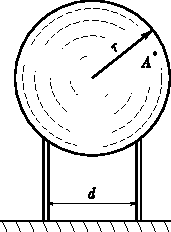
\includegraphics{figure/fig01.32}
        \caption{}
        \label{fig:01.32}
    \end{center}
\end{figurex}